\documentclass[10pt, a4paper]{article}

% On écrit en français
\usepackage[utf8]{inputenc}
\usepackage[frenchb]{babel}
\usepackage[T1]{fontenc}

% Packages nécessaires
\usepackage{graphicx}
\usepackage{hyperref}

% Numérotation de page custom
\usepackage{fancyhdr}
\usepackage{lastpage}
\pagestyle{fancy}
\fancyhf{}
\rfoot{Page \thepage \hspace{1pt} sur \pageref{LastPage}}

% Police Helvetica <3
\usepackage{helvet}
\renewcommand*{\familydefault}{\sfdefault}

% Enlever les alinéas
\setlength{\parindent}{0pt}

% Marges plus larges pour faire moins LaTeX
\usepackage[left=3cm, right=3cm]{geometry}

% Sous titre de document
\usepackage{titling}
\newcommand{\subtitle}[1]{%
  \posttitle{%
    \par\end{center}
    \begin{center}\large#1\end{center}
    \vskip0.5em}%
}

% En tête complet de document
\newcommand{\Document}[1]{%
    \title{#1}
    \subtitle{Dématérialisation d'un processus de paiement}
    \author{
        COMETS Jean-Marie \\
        DELMARRE Adrian \\
        REYNOLDS Nicolas \\
        TURPIN Pierre
    }
    \date{\today}

    \maketitle \newpage

    \tableofcontents \newpage
}

\usepackage{rotating}

\begin{document}

\Document{Architecture applicative}

\section{Définition des objets métiers}

La figure \ref{fig:mcd} est le MCD (Modèle Conceptuel de Données) global du
système. Il recense toutes les données utilisées dans le système d'information
de l'étude. \\

Les échanges liés au marketing ne figurent pas dans le MCD comme les commandes
ou même les factures (lesquelles existent dans le modèle en tant que commandes
échues amenant une transaction certaine). Lorsqu'une entreprise est approchée
par le service marketing, elle est référencée en base et acquiert le statut de
"prospect". Lorsqu'elle signe son premier contrat avec nous, son statut devient
alors "prospect". Les informations relatives au contact (et à l'éventuel refus
essuyé) sortent du champ de granularité observé. \\

Il en est de même pour les transactions bancaires. L'acteur Banque a un simple
rôle de garant des transactions :

\begin{itemize}
  \item La banque XXX partenaire d'AVENTIX garantit les transactions des bornes
    NFC auprès des commerçants qui les hébergent. Ce mouvement permet de
    différer et mutualiser le débit effectif.
  \item La banque XXX partenaire d'AVENTIX garantit les transactions induites
    par l'achat de crédit, que ce soit par un utilisateur final, ou par une
    entreprise. Dans les deux cas, cette garantie se fait de connivence avec la
    banque respective de l'acteur concerné.
\end{itemize}

La contrainte d'exclusion modélisée sur la relation de contact symbolise le
fait qu'une action de contact ne peut concerner qu'un type d'acteur à la fois.

\begin{landscape}
  \begin{figure}[ht]
      \centering
      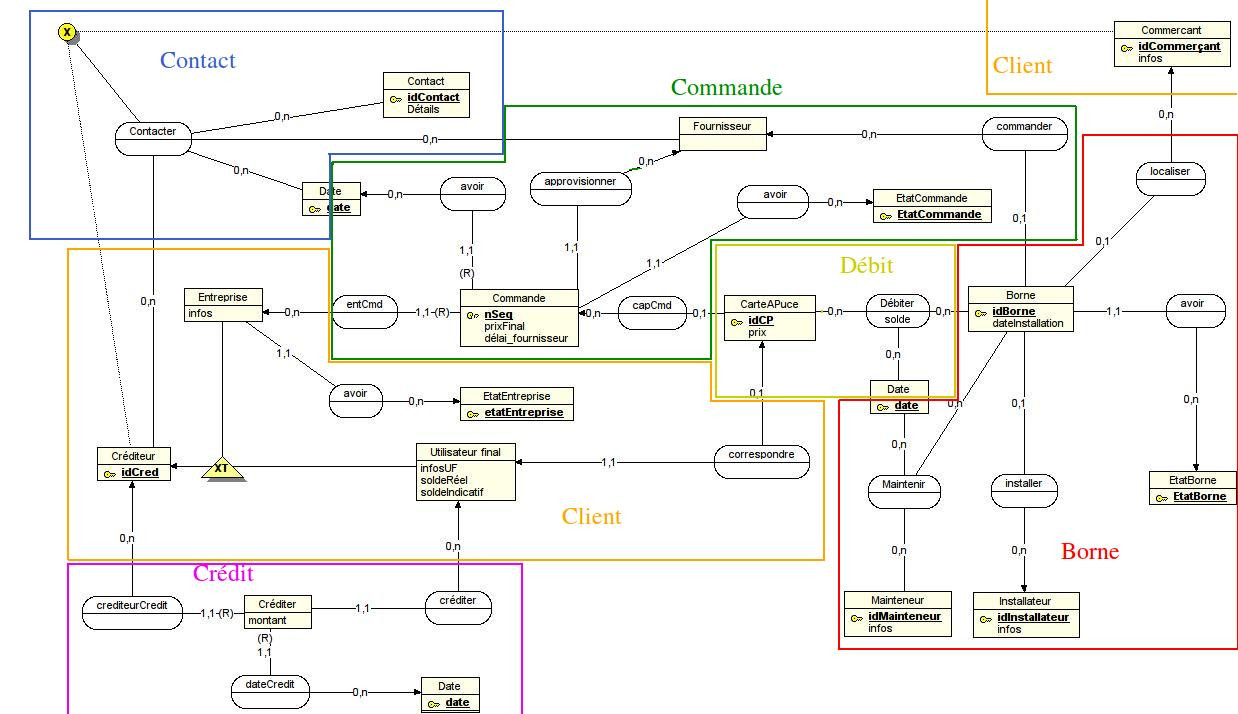
\includegraphics[width=0.7\paperheight]{mcd}
      \caption{MCD global du système}
      \label{fig:mcd}
  \end{figure}
\end{landscape}

Les objets métiers utilisés dans la solution sont les suivants : \\

\begin{description}
  \item[Contact] contact effectué avec une entreprise, historisant les
    différents contacts qui ont été pris (marketing, support, etc).
  \item[Commande] action de commande de cartes à puce par l'entreprise.
  \item[État d'une commande] une commande pourra être dans un des états
    suivants :
    \begin{itemize}
      \item débutée
      \item prise en charge
      \item en attente de fournisseur
      \item en cours de livraison
      \item annulée
      \item finie
    \end{itemize}
  \item[Carte à puce] carte numérique identifiable par un numéro unique,
    communiquant avec une borne pour effectuer un paiement.
  \item[Borne] borne pouvant lire des cartes à puce
  \item[État d'une borne] une borne pourra être dans un des états suivants :
    \begin{itemize}
      \item en stock
      \item installée
      \item fonctionnelle
      \item en panne
      \item ne communique pas
      \item en réparation
    \end{itemize}
  \item[Fournisseur] agent externe servant à fournir le système en cartes à
    puce ou en borne. Aucune distinction n'est faite entre ces deux vu que
    c'est le même service qui va gérer les commandes de chaque.
  \item[Entreprise] entreprise employant des utilisateurs finals, pouvant
    commander des cartes à puce et créditer des utilisateurs finaux.
  \item[État d'une entreprise] une entreprise pourra être dans un des états suivants :
    \begin{itemize}
      \item prospect
      \item client
    \end{itemize}
  \item[Utilisateur final] utilisateur de la carte à puce, faisant ses achats
    chez des commerçants, et travaillant au sein d'une entreprise.
  \item[Créditeur] personne capable de créditer un utilisateur final. Il peut
    s'agir d'une entreprise ou d'un utilisateur final.
  \item[Commercant] agent externe pouvant accueillir une borne, pouvant ainsi
    effectuer des ventes depuis celle-ci.
  \item[Mainteneur] acteur externe responsable de la maintenance d'une borne
    chez un commerçant.
  \item[Installateur] acteur externe responsable de l'installation d'une borne
    chez un commerçant. Il peut aussi être un mainteneur, mais pas forcément,
    d'où la distinction entre chacun.
\end{description}

Bien entendu, l'objet \textbf{Date} concerne l'historisation d'une action, et
n'est représenté que par rigueur. Chaque date est identifiable uniquement par
son temps \textbf{EPOCH}, le nombre de secondes s'étant écoulées depuis le
\textbf{Jeudi 1\textsuperscript{er} Janvier 1970, 00:00 UTC}.

\section{Extraction des blocs fonctionnels}

À partir du MCD \ref{fig:mcd}, 6 blocs fonctionnels ont été retenu :

\begin{description}
  \item[Contacts] exposition du système aux acteurs externes, et concerne
    surtout le support (maintenance).
  \item[Clients] ensemble des acteurs externes et leur interconnexions, ce bloc
    a été choisi par sémantique plutôt que par cohérence fonctionnelle.
  \item[Commande] concerne les commandes de cartes à puce par l'entreprise.
  \item[Borne] fonctionnement et maintenance des bornes correspondantes aux
    cartes à puce.
  \item[Débit] actions de débit d'un utilisateur final
  \item[Crédit] actions de crédit d'un utilisateur final
\end{description}

% TODO plus de détails sur les blocs, eg PIPEAU

\section{Listing des applications utilisateurs}

Le découpage applicatif le plus pertinent est un découpage par type de client.
Les usages sont variés en fonction de l'acteur, et cela donne au client une
interface unique. Également, les règles de suivi varient d'un acteur à
l'autre.\\

Nous avons alors 3 acteurs principaux dans l'étude ce qui donne 3 applications
utilisateurs : \\
\begin{itemize}
  \item Application de gestion d'un commerçant
  \item Application de gestion d'une entreprise
  \item Application de gestion d'un utilisateur final
\end{itemize}
~\\

\CUBref
{Application de gestion d'un commerçant}
{
  Cette application permet principalement aux commerçant de gérer et visualiser
  leurs transactions effectuées en utilisant ce système. \\

  Il permet également aux commerçant de signaler si un problème à eu lieu
  durant l'utilisation du système, ou si il y a eu une erreur après
  l'utilisation. \\
}
{Commerçant}
{
  Le commerçant doit être inscrit comme un commerçant auprès d'Aventix et donc
  avoir une ou plusieurs bornes. \\

  Les actions qu'il peut effectuées sont disponible uniquement grâce à une
  identification sur l'IHM des services métiers correspondants (sauf mention
  contraire explicite sur un des services métier). \\

  Les identifiants à fournir pour s'authentifier sont établies durant
  l'enregistrement du commerçant dans le SI. \\
}
{Pas de conséquences}
{
  \begin{itemize}
    \item Le commerçant n'est pas authentifié lorsqu'il essaye d'utiliser un
      service nécessitant une authentification. Il est alors simplement redirigé
      vers la connexion.
  \end{itemize}
}

\CUBref
{Application de gestion d'une entreprise}
{
  Cette application permet principalement aux entreprises de gérer leurs
  employés en tant qu'utilisateurs finaux dans le SI. \\

  L'entreprise peut effectuer des requêtes pour créer ou supprimer un
  utilisateur. \\

  Il peut aussi décider de désactiver un de ses employées temporairement ce qui
  permet de gérer les cas où les titres-restaurant sont pas utilisables (en
  vacances par exemple). L'entreprise a, bien sur, la possibilité de réactiver
  un de ses employés. \\

  L'ajout de crédits mensuelles dans les comptes de ses employés est à la
  charge de l'entreprise. Elle possède donc un moyen de créditer ses propres
  employés. \\

  Il permet également aux entreprises de signaler si un problème à eu lieu
  durant l'utilisation du système. \\
}
{Entreprise}
{
  L'entreprise doit être inscrit comme une entreprise auprès d'Aventix. \\

  Les actions qu'il peut effectuées sont disponible uniquement grâce à une
  identification sur l'IHM des services métiers correspondants (sauf mention
  contraire explicite sur un des services métier). \\

  Les identifiants à fournir pour s'authentifier sont établies durant
  l'enregistrement de l'entreprise dans le SI. \\
}
{Pas de conséquences}
{
  \begin{itemize}
    \item L'entreprise n'est pas authentifié lorsqu'il essaye d'utiliser un
      service nécessitant une authentification. Elle est alors simplement
      redirigé vers la connexion.
  \end{itemize}
}

\CUBref
{Application de gestion d'un utilisateur final}
{
  Cette application permet principalement aux utilisateurs finaux de gérer leurs
  crédits sur leur carte à puce. \\

  Il peuvent consulter l'état du compte de leur carte à puce. \\

  En tant que personne morale souscrivant à un service, il a le droit de
  modifier ses données personnelles enregistrées. \\

  Afin de pouvoir utiliser la carte à puce en dehors des limites de crédits
  imposées par son entreprise, l'utilisateur final peut se créditer lui-même. \\

  L'application permet également aux utilisateurs finaux de signaler si un
  problème à eu lieu durant l'utilisation du système. \\
}
{Utilisateur final}
{
  L'utilisateur doit être inscrit et actif auprès d'Aventix. \\

  Les actions qu'il peut effectuées sont disponible uniquement grâce à une
  identification sur l'IHM des services métiers correspondants (sauf mention
  contraire explicite sur un des services métier). \\

  Les identifiants à fournir pour s'authentifier sont établies durant
  la création de l'utilisateur final par l'entreprise dans le SI. \\
}
{Pas de conséquences}
{
  \begin{itemize}
    \item L'utilisateur final n'est pas authentifié lorsqu'il essaye d'utiliser
      un service nécessitant une authentification. Il est alors simplement
      redirigé vers la connexion.
  \end{itemize}
}

\section{Génération des services}
\subsection{Services applicatif}
La liste des services applicatifs est la suivante : \\
\begin{itemize}
  \item Application de gestion d'un commerçant
  \item Application de gestion d'une entreprise
  \item Application de gestion d'un utilisateur final
\end{itemize}
~\\

\subsection{Services métier}
% Un commerçant peut signaler une panne à Aventix. Celle-ci doivent être
% enregistrer dans le SI afin d'améliorer la qualité du produit et tracer les
% éventuelles erreurs. \\
% 
% Un commerçant à le droit de visualiser et suivre les transactions physiques
% utilisant les services de la solution. Les transactions sont enregistrées dans
% le SI et un commerçant habilité doit pouvoir avoir accès à celles-ci. \\

% TODO récupérer les services métier utilisés dans les DSD et les noter ici,
% peut-être avec une description.

\subsubsection{Contacts}
% \begin{description}
% \end{description}

\subsubsection{Clients}
\begin{description}
  \item[setInfosUF(id, infos)] Met à jour les informations personnelles de l'utilisateur final
  \item[loginUF(loginInfos)] Tentative de connexion de l'utilisateur final avec ses informations de connexion
  \item[connectUF(loginInfos)] Connexion effective de l'utlisateur dans le système
  \item[activateUF(idUF)] Activation de l'utilisateur final l'autorisant à effectuer des opérations
  \item[deactivateUF(idUF)] Désactivation de l'utlisateur final l'interdisant à effectuer des opérations
  \item[notifyUF(infosUF, body)] Envoie d'un message à l'utilisateur final selon le corpus spécifié
  \item[create(infosUF)] Création d'un nouvel utilisateur final au sein du SI en utilisant les informations
  \item[remove(idUF)] Suppression d'un utilisateur final
  \item[checkInfosUF(infosUF)] Vérification de l'intégrité sémantique des données
  \item[loginCommerçant(loginInfos)] Tentative de connexion d'un commerçant avec ses informations de connexion
  \item[connectCommerçant(loginInfos)] Connexion effective d'un commerçant dans le système
  \item[loginEntreprise(loginInfos)] Tentative de connexion d'une entreprise avec ses informations de connexion
  \item[connectEntreprise(loginInfos)] Connexion effective d'une entreprise dans le système
\end{description}

\subsubsection{Débit}
% \begin{description}
% \end{description}

\subsubsection{Crédit}
% \begin{description}
% \end{description}

% TODO faire la partie des BF Borne et Commande

\subsection{Services objet métier}
Toutes les opérations des services objet métier suivent le formalise
\textbf{CRUD}. C'est pourquoi, nous ne les listons et ne les détaillons pas
ici. \\

\section{Mise en application des services}
Malgré la similarité entre les trois diagrammes de séquence
\ref{dsd:connect-uf}, \ref{dsd:connect-com} et \ref{dsd:connect-comp}, nous
avons décidé de les inclure au vu des différences au niveau des services métier
et objet métier.

% DSD: modification des informations de l'utilisateur final
\begin{figure}
  \centering

  \begin{sequencediagram}
      \newthread{acteur}{Acteur~:~Utilisateur final}
      \newinst{ihm}{IHM}
      \newinst{sm}{SM~:~Clients}
      \newinst{som}{SOM~:~Utilisateur final}

      \begin{call}{acteur}{submit(idUF, infosUF)}{ihm}{confirmation}
          \begin{messcall}{ihm}{setInfosUF(id, infos)}{sm}
            \begin{call}{sm}{findById(id)}{som}{found}
            \end{call}
            \begin{sdblock}{IF}{found = TRUE}
              \begin{callself}{sm}{checkInfosUF(infos)}{status,~message}
              \end{callself}
              \begin{sdblock}{IF}{status = OK}
                \begin{call}{sm}{setInfos(id, infos)}{som}{}
                \end{call}
                \begin{mess}{sm}{OK, ACCEPTED}{ihm}
                \end{mess}
              \end{sdblock}
              \begin{sdblock}{ELSE}{status != OK}
                \begin{mess}{sm}{NOT OK, message}{ihm}
                \end{mess}
              \end{sdblock}
            \end{sdblock}
            \begin{sdblock}{ELSE}{found != TRUE}
                \begin{mess}{sm}{NOT OK, NOT FOUND}{ihm}
                \end{mess}
            \end{sdblock}
          \end{messcall}
      \end{call}
  \end{sequencediagram}

  \caption{Modification des informations de l'utilisateur final}
  \label{dsd:set-infos-uf}
\end{figure}

% DSD: connexion de l'utilisateur final
\begin{figure}
  \centering

  \begin{sequencediagram}
      \newthread{acteur}{Acteur~:~Utilisateur final}
      \newinst{ihm}{IHM}
      \newinst{sm}{SM~:~Clients}
      \newinst{som}{SOM~:~Utilisateur final}

      \begin{call}{acteur}{submit(loginInfos)}{ihm}{confirmation}
          \begin{messcall}{ihm}{loginUF(loginInfos)}{sm}
            \begin{call}{sm}{findByLoginInfos(loginsInfos)}{som}{id, found, activated}
            \end{call}
            \begin{sdblock}{IF}{found = TRUE and activated = TRUE}
              \begin{callself}{sm}{connectUF(id)}{}
              \end{callself}
              \begin{mess}{sm}{OK}{ihm}
              \end{mess}
            \end{sdblock}
            \begin{sdblock}{ELSE}{found != TRUE or activated != TRUE}
                \begin{mess}{sm}{NOT OK}{ihm}
                \end{mess}
            \end{sdblock}
          \end{messcall}
      \end{call}
  \end{sequencediagram}

  \caption{Connexion de l'utilisateur final}
  \label{dsd:connect-uf}
\end{figure}

% DSD: activation d'un utilisateur final
\begin{figure}
  \centering

  \begin{sequencediagram}
      \newthread{acteur}{Acteur~:~Entreprise}
      \newinst{ihm}{IHM}
      \newinst{sm}{SM~:~Clients}
      \newinst{som}{SOM~:~Utilisateur final}

      \begin{call}{acteur}{submit(idUF)}{ihm}{confirmation}
          \begin{messcall}{ihm}{activateUF(idUF)}{sm}
            \begin{call}{sm}{findById(idUF)}{som}{found}
            \end{call}
            \begin{sdblock}{IF}{found = TRUE}
              \begin{call}{sm}{activate(idUF)}{som}{}
              \end{call}
              \begin{callself}{sm}{notifyUF(idUF, ACTIVATION)}{}
              \end{callself}
              \begin{mess}{sm}{OK}{ihm}
              \end{mess}
            \end{sdblock}
            \begin{sdblock}{ELSE}{found != TRUE}
                \begin{mess}{sm}{NOT OK}{ihm}
                \end{mess}
            \end{sdblock}
          \end{messcall}
      \end{call}
  \end{sequencediagram}

  \caption{Activation d'un utilisateur final}
  \label{dsd:activate-uf}
\end{figure}

% DSD: desactivation d'un utilisateur final
\begin{figure}
  \centering

  \begin{sequencediagram}
      \newthread{acteur}{Acteur~:~Entreprise}
      \newinst{ihm}{IHM}
      \newinst{sm}{SM~:~Clients}
      \newinst{som}{SOM~:~Utilisateur final}

      \begin{call}{acteur}{submit(idUF)}{ihm}{confirmation}
          \begin{messcall}{ihm}{deactivateUF(idUF)}{sm}
            \begin{call}{sm}{findById(idUF)}{som}{found}
            \end{call}
            \begin{sdblock}{IF}{found = TRUE}
              \begin{call}{sm}{deactivate(idUF)}{som}{}
              \end{call}
              \begin{callself}{sm}{notifyUF(idUF, DEACTIVATION)}{}
              \end{callself}
              \begin{mess}{sm}{OK}{ihm}
              \end{mess}
            \end{sdblock}
            \begin{sdblock}{ELSE}{found != TRUE}
                \begin{mess}{sm}{NOT OK}{ihm}
                \end{mess}
            \end{sdblock}
          \end{messcall}
      \end{call}
  \end{sequencediagram}

  \caption{Desactivation d'un utilisateur final}
  \label{dsd:deactivate-uf}
\end{figure}

% DSD: création d'un utilisateur final
\begin{figure}
  \centering

  \resizebox{!}{0.85\totalheight}{\begin{sequencediagram}
      \newthread{acteur}{Acteur~:~Entreprise}
      \newinst{ihm}{IHM}
      \newinst{sm}{SM~:~Clients}
      \newinst{som}{SOM~:~Utilisateur final}
      \newinst{api}{API~:~Banque}

      \begin{call}{acteur}{submit(infosUF)}{ihm}{confirmation}
          \begin{messcall}{ihm}{createUF(infosUF)}{sm}
            \begin{call}{sm}{findByInfos(infoUF)}{som}{found}
            \end{call}
            \begin{sdblock}{IF}{found = TRUE}
              \begin{mess}{sm}{NOT OK, ALREADY EXIST}{ihm}
              \end{mess}
            \end{sdblock}
            \begin{sdblock}{ELSE}{found != TRUE}
              \begin{callself}{sm}{checkInfosUF(infosUF)}{status, message}
              \end{callself}
              \begin{sdblock}{IF}{status = OK}
                \begin{call}{sm}{create(infosUF)}{som}{id}
                \end{call}
                \begin{call}{sm}{createAccountUF(id)}{api}{status}
                \end{call}
                \begin{sdblock}{IF}{status = OK}
                  \begin{mess}{sm}{OK}{ihm}
                  \end{mess}
                \end{sdblock}
                \begin{sdblock}{ELSE}{status != OK}
                  \begin{messcall}{sm}{remove(id)}{som}
                  \end{messcall}
                  \begin{mess}{sm}{NOT OK}{ihm}
                  \end{mess}
                \end{sdblock}
              \end{sdblock}
              \begin{sdblock}{ELSE}{status != OK}
                \begin{mess}{sm}{NOT OK}{ihm}
                \end{mess}
              \end{sdblock}
            \end{sdblock}
          \end{messcall}
      \end{call}
  \end{sequencediagram}}

  \caption{Création d'un utilisateur final}
  \label{dsd:create-uf}
\end{figure}

% DSD: supprimer un utilisateur final
\begin{figure}
  \centering

  \resizebox{!}{0.85\totalheight}{\begin{sequencediagram}
      \newthread{acteur}{Acteur~:~Entreprise}
      \newinst{ihm}{IHM}
      \newinst{sm}{SM~:~Clients}
      \newinst{som}{SOM~:~Utilisateur final}
      \newinst{api}{API~:~Banque}

      \begin{call}{acteur}{submit(idUF)}{ihm}{removed}
        \begin{call}{ihm}{removeUF(idUF)}{sm}{removed}
          \begin{call}{sm}{removeById(idUF)}{som}{removed}
          \end{call}
          \begin{sdblock}{IF}{removed = TRUE}
            \begin{messcall}{sm}{removeAccountUF(idUF)}{api}
            \end{messcall}
          \end{sdblock}
        \end{call}
      \end{call}
  \end{sequencediagram}}

  \caption{Suppression d'un utilisateur final}
  \label{dsd:remove-uf}
\end{figure}

% DSD: connexion d'un commerçant
\begin{figure}
  \centering

  \begin{sequencediagram}
      \newthread{acteur}{Acteur~:~Commerçant}
      \newinst{ihm}{IHM}
      \newinst{sm}{SM~:~Clients}
      \newinst{som}{SOM~:~Commerçant}

      \begin{call}{acteur}{submit(loginInfos)}{ihm}{confirmation}
          \begin{messcall}{ihm}{loginCommerçant(loginInfos)}{sm}
            \begin{call}{sm}{findByLoginInfos(loginsInfos)}{som}{id, found}
            \end{call}
            \begin{sdblock}{IF}{found = TRUE}
              \begin{callself}{sm}{connectCommerçant(id)}{}
              \end{callself}
              \begin{mess}{sm}{OK}{ihm}
              \end{mess}
            \end{sdblock}
            \begin{sdblock}{ELSE}{found != TRUE}
                \begin{mess}{sm}{NOT OK}{ihm}
                \end{mess}
            \end{sdblock}
          \end{messcall}
      \end{call}
  \end{sequencediagram}

  \caption{Connexion d'un commerçant}
  \label{dsd:connect-com}
\end{figure}

% DSD: connexion d'une entreprise
\begin{figure}
  \centering

  \begin{sequencediagram}
      \newthread{acteur}{Acteur~:~Entreprise}
      \newinst{ihm}{IHM}
      \newinst{sm}{SM~:~Clients}
      \newinst{som}{SOM~:~Entreprise}

      \begin{call}{acteur}{submit(loginInfos)}{ihm}{confirmation}
          \begin{messcall}{ihm}{loginEntreprise(loginInfos)}{sm}
            \begin{call}{sm}{findByLoginInfos(loginsInfos)}{som}{id, found}
            \end{call}
            \begin{sdblock}{IF}{found = TRUE}
              \begin{callself}{sm}{connectEntreprise(id)}{}
              \end{callself}
              \begin{mess}{sm}{OK}{ihm}
              \end{mess}
            \end{sdblock}
            \begin{sdblock}{ELSE}{found != TRUE}
                \begin{mess}{sm}{NOT OK}{ihm}
                \end{mess}
            \end{sdblock}
          \end{messcall}
      \end{call}
  \end{sequencediagram}

  \caption{Connexion d'un entreprise}
  \label{dsd:connect-comp}
\end{figure}

% DSD signaler problème commerçant
\begin{landscape}
  \begin{figure}
    \centering

    \begin{sequencediagram}
        \newthread{acteur}{Acteur~:~Commerçant}
        \newinst{ihm}{IHM}
        \newinst{sm}{SM~:~Contacts}
        \newinst{somb}{SOM~:~Borne}
        \newinst{somc}{SOM~:~Contact}
        \newinst{somcom}{SOM~:~Commerçant}

        \begin{call}{acteur}{submit(idCommerçant, idBorne, infosMessage)}{ihm}{confirmation}
            \begin{messcall}{ihm}{reportCommerçant(idCommerçant, idBorne, infosMessage)}{sm}
              \begin{call}{sm}{findById(idBorne)}{somb}{id, foundBorne}
              \end{call}
              \begin{call}{sm}{findById(idCommerçant)}{somcom}{id, foundCommerçant}
              \end{call}
              \begin{sdblock}{IF}{foundBorne = TRUE AND foundCommerçant = TRUE}
                \begin{mess}{sm}{reportCommerçant(idCommerçant, idBorne, infosMessage)}{somc}
                \end{mess}
                \begin{mess}{sm}{OK}{ihm}
                \end{mess}
              \end{sdblock}
              \begin{sdblock}{ELSE}{foundBorne != TRUE OR foundCommerçant != TRUE}
                  \begin{mess}{sm}{NOT OK, NOT FOUND}{ihm}
                  \end{mess}
              \end{sdblock}
            \end{messcall}
        \end{call}
    \end{sequencediagram}

    \caption{Commerçant qui signale un poblème}
    \label{dsd:signal-com}
  \end{figure}
\end{landscape}

% DSD signaler problème entreprise
\begin{figure}
  \centering

  \begin{sequencediagram}
      \newthread{acteur}{Acteur~:~Entreprise}
      \newinst{ihm}{IHM}
      \newinst{sm}{SM~:~Contacts}
      \newinst{somc}{SOM~:~Contact}
      \newinst{some}{SOM~:~Entreprise}

      \begin{call}{acteur}{submit(idEntreprise, infosMessage)}{ihm}{confirmation}
          \begin{messcall}{ihm}{reportEntreprise(idEntreprise, infosMessage)}{sm}
            \begin{call}{sm}{findById(idEntreprise)}{some}{id, foundEntreprise}
            \end{call}
            \begin{sdblock}{IF}{foundEntreprise = TRUE}
              \begin{mess}{sm}{reportEntreprise(idEntreprise, infosMessage)}{somc}
              \end{mess}
              \begin{mess}{sm}{OK}{ihm}
              \end{mess}
            \end{sdblock}
            \begin{sdblock}{ELSE}{foundEntreprise != TRUE}
                \begin{mess}{sm}{NOT OK, NOT FOUND}{ihm}
                \end{mess}
            \end{sdblock}
          \end{messcall}
      \end{call}
  \end{sequencediagram}

  \caption{Entreprise qui signale un poblème}
  \label{dsd:signal-comp}
\end{figure}

% DSD signaler problème UF
\begin{figure}
  \centering

  \begin{sequencediagram}
      \newthread{acteur}{Acteur~:~Utilisateur final}
      \newinst{ihm}{IHM}
      \newinst{sm}{SM~:~Contacts}
      \newinst{somc}{SOM~:~Contact}
      \newinst{somu}{SOM~:~Utilisateur final}

      \begin{call}{acteur}{submit(idUF, infosMessage)}{ihm}{confirmation}
          \begin{messcall}{ihm}{reportUF(idUF, infosMessage)}{sm}
            \begin{call}{sm}{findById(idUF)}{somu}{id, foundUF}
            \end{call}
            \begin{sdblock}{IF}{foundUF = TRUE}
              \begin{mess}{sm}{reportUF(idUF, infosMessage)}{somc}
              \end{mess}
              \begin{mess}{sm}{OK}{ihm}
              \end{mess}
            \end{sdblock}
            \begin{sdblock}{ELSE}{foundUF != TRUE}
                \begin{mess}{sm}{NOT OK, NOT FOUND}{ihm}
                \end{mess}
            \end{sdblock}
          \end{messcall}
      \end{call}
  \end{sequencediagram}

  \caption{Utilisateur final qui signale un poblème}
  \label{dsd:signal-uf}
\end{figure}

\end{document}

% vim: ft=tex et sw=2 sts=2
